\section{Visi\'on general del sistema}

Este diagrama respresenta la interacci\'on entre los diferentes elementos de hardware 
y software en una experiencia planificada.

\begin{figure}[!htb].
    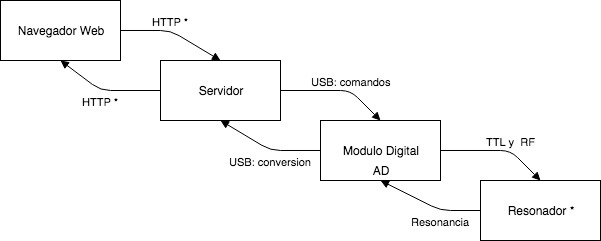
\includegraphics[width=\linewidth]{../figures/d5.jpg}
    \caption{Visi\'on General del sistema}
    \label{fig:d5}
\end{figure}

\subsection{Navegador web}
El navegador web es la plataforma donde se provee al usuario final la interfaz con el sistema.

\subsection{Servidor}
El servidor provee servicios REST solicitados por la interfaz gr\'afica durante la vida
de la sesi\'on del usuario. Estos servicios hacen llamadas al controlador del M\'odulo
Digital via usb.

\subsection{M\'odulo Digital}
El m\'odulo digital procesa los mensajes del controlador via usb y ejecuta 
el microc\'odigo del mismo para la configuraci\'on y ejecuci\'on de las secuencias de pulsos.

\subsection{Resonador}
El resonador recibe los pulsos provenientes del M\'odulo Digital generando una se\~nal de resonancia
enviada al M\'odulo Digital para su conversi\'on digital.

\newpage